
\subsection{Quantum Gates and Circuits}
\label{subsec:gates}

\begin{definition}[Quantum Gate]
A \emph{quantum gate} is a unitary operator \(U\) acting on a quantum state, meaning that \(U^\dagger U = I\). Quantum gates manipulate \glspl{qubit} and form the basic operations in quantum circuits.
\end{definition}

\begin{notation}[Single-Qubit Gates]
Key single-qubit gates include:
\begin{itemize}
    \item \textbf{Pauli-X (bit-flip):}
    \[
    X = \begin{pmatrix} 0 & 1 \\ 1 & 0 \end{pmatrix},
    \]
    which performs \(X|0\rangle = |1\rangle\) and \(X|1\rangle = |0\rangle\).
    \item \textbf{Hadamard:}
    \[
    H = \frac{1}{\sqrt{2}}\begin{pmatrix} 1 & 1 \\ 1 & -1 \end{pmatrix},
    \]
    creating superpositions as seen in the previous section.
    \item \textbf{Phase Shift:}
    \[
    R_\phi = \begin{pmatrix} 1 & 0 \\ 0 & e^{i\phi} \end{pmatrix}.
    \]
\end{itemize}
\end{notation}

\begin{definition}[Two-Qubit Gate]
A two-qubit gate, such as the \gls{cnot} gate, acts on a pair of qubits. The \gls{cnot} gate flips the second (target) qubit if the first (control) qubit is \(|1\rangle\); formally,
\[
\text{CNOT}|a\rangle|b\rangle = |a\rangle|a \oplus b\rangle,
\]
where \(\oplus\) denotes addition modulo 2.
\end{definition}

\begin{remark}
A universal set of quantum gates, for example \(\{H, T, \gls{cnot}\}\), can approximate any unitary operation to arbitrary precision, thereby forming the foundation of the quantum circuit model.
\end{remark}

\begin{example}[Deutsch-Jozsa Quantum Circuit]
Figure~\ref{fig:deutsch_circuit} shows a quantum circuit used in the Deutsch-Jozsa algorithm. The circuit demonstrates the application of Hadamard gates before and after the oracle \(U_f\), highlighting the interplay of superposition and entanglement in quantum computation.
\end{example}

\begin{figure}[h]
\centering
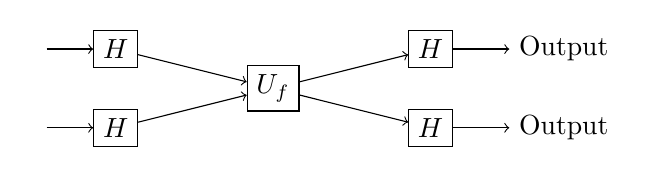
\begin{tikzpicture}[node distance=1.8cm, auto]
    \node (in1) at (0,0) {};
    \node (in2) at (0,-1) {};
    \node[draw, rectangle] (H1) at (1,0) {$H$};
    \node[draw, rectangle] (H2) at (1,-1) {$H$};
    \node[draw, rectangle] (Uf) at (3, -0.5) {\(U_f\)};
    \node[draw, rectangle] (H3) at (5,0) {$H$};
    \node[draw, rectangle] (H4) at (5,-1) {$H$};
    \draw[->] (in1) -- (H1);
    \draw[->] (in2) -- (H2);
    \draw[->] (H1) -- (Uf);
    \draw[->] (H2) -- (Uf);
    \draw[->] (Uf) -- (H3);
    \draw[->] (Uf) -- (H4);
    \draw[->] (H3) -- ++(1,0) node[right] {Output};
    \draw[->] (H4) -- ++(1,0) node[right] {Output};
\end{tikzpicture}
\caption{Quantum circuit for the Deutsch-Jozsa algorithm.}
\label{fig:deutsch_circuit}
\end{figure}